\documentclass{article}
\usepackage{amsmath, amssymb}
\usepackage{tikz}
\usepackage{graphicx}
\usepackage{caption}
\usepackage[margin=1in, landscape]{geometry}
\usetikzlibrary{shapes, arrows, positioning, fit, calc}

\begin{document}

\noindent
\resizebox{\linewidth}{!}{%
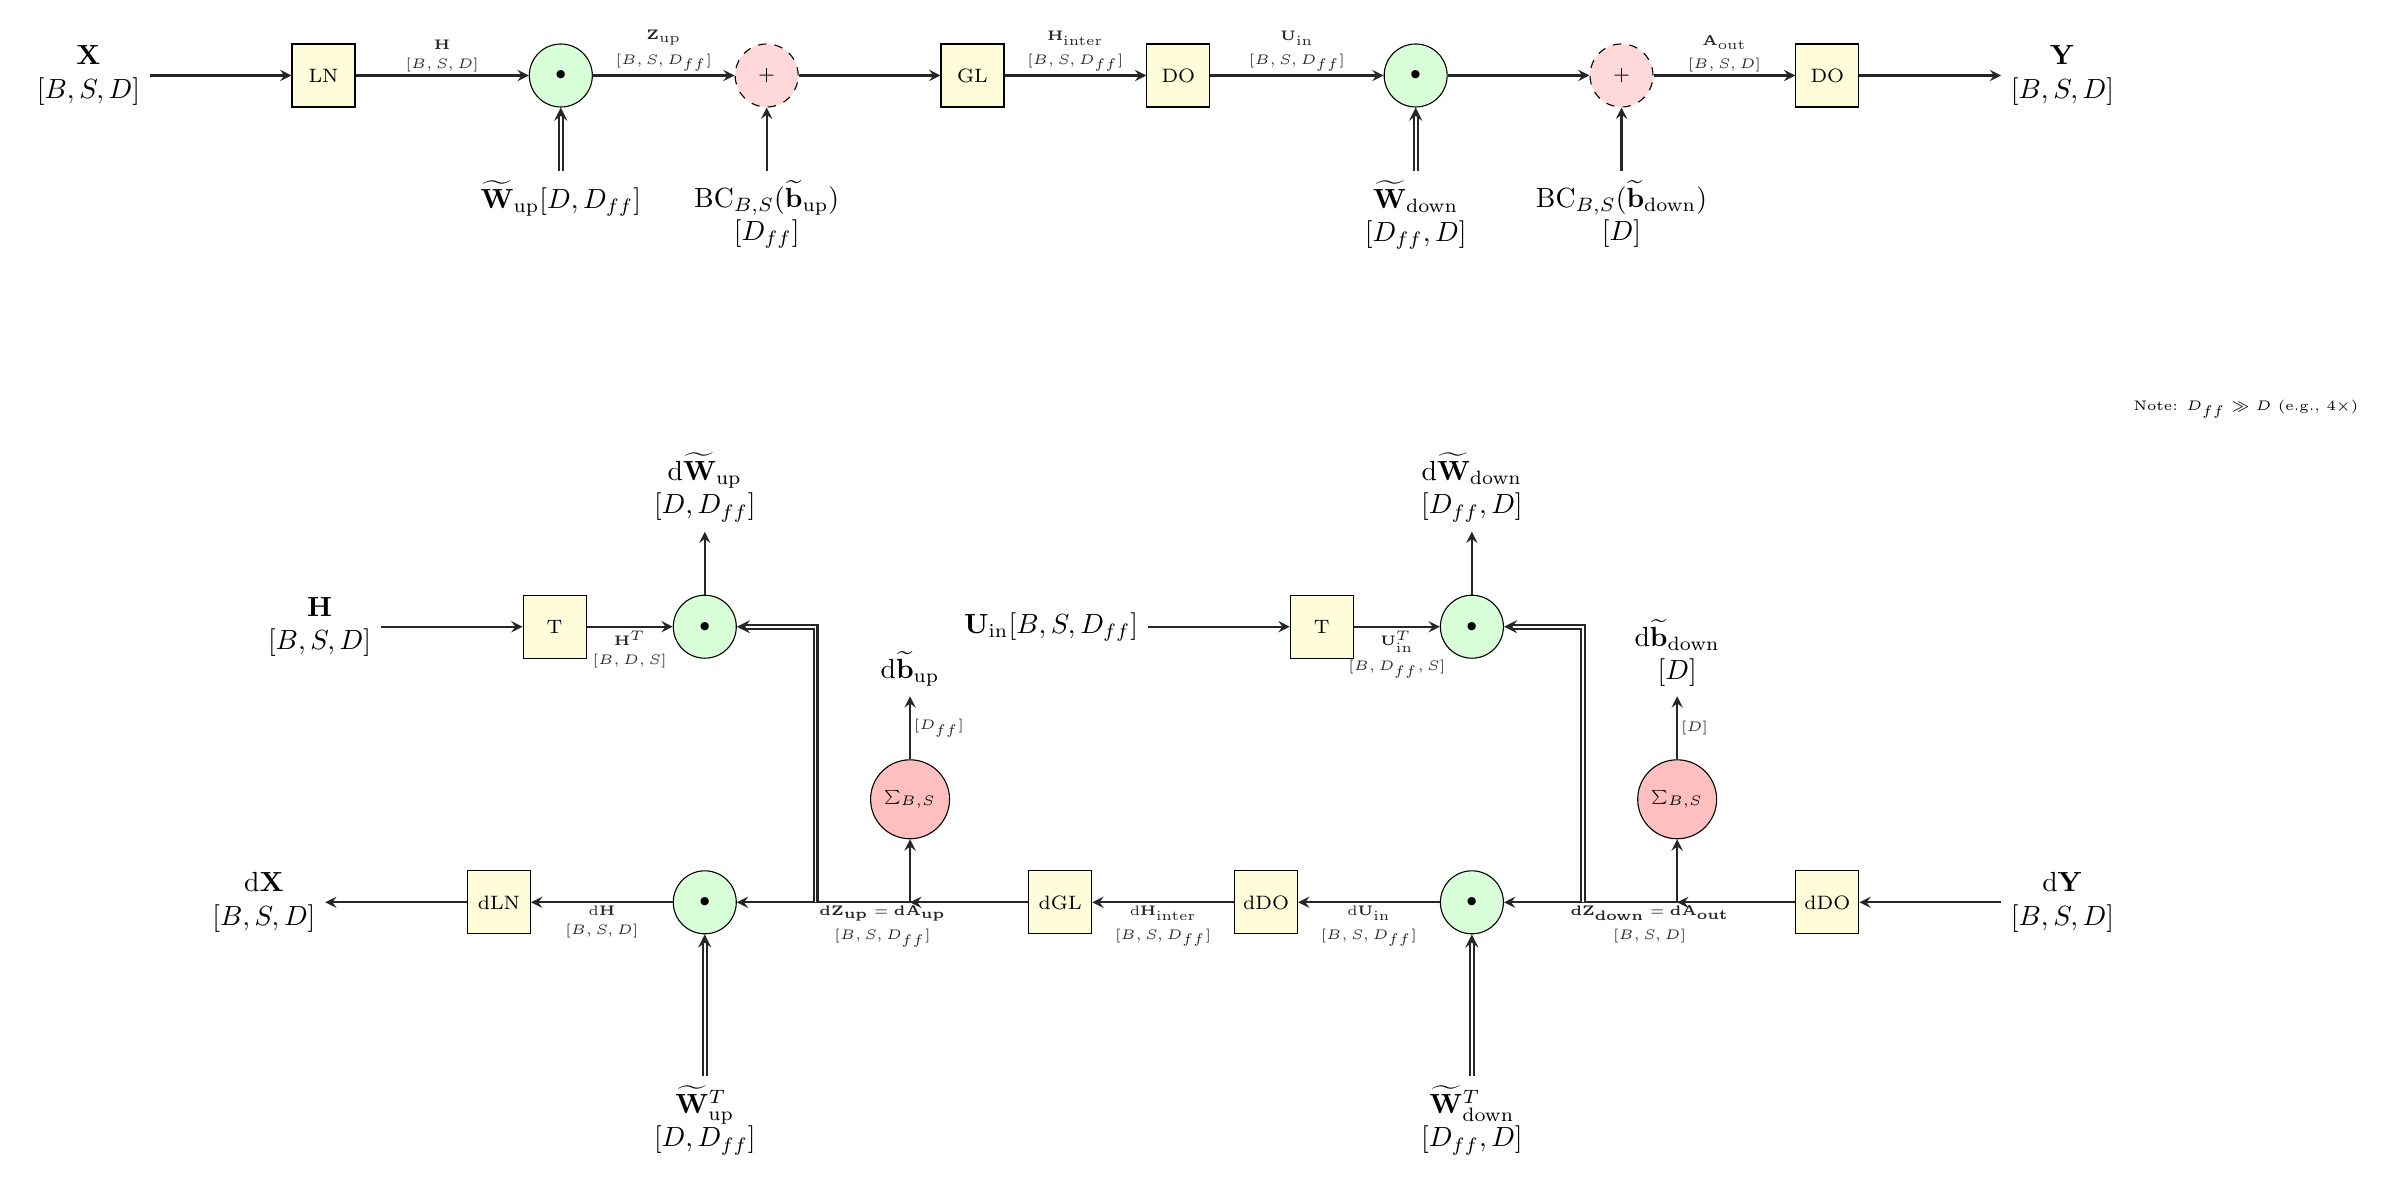
\begin{tikzpicture}[
    >=stealth,
    % --- NODE STYLES ---
    auxnode/.style={draw, rectangle, fill=yellow!15, minimum height=8mm, minimum width=8mm, inner sep=2pt, font=\scriptsize, align=center},
    mulnode/.style={draw, circle, fill=green!15, minimum size=8mm, font=\scriptsize, align=center},
    addnode/.style={draw, circle, dashed, fill=red!15, minimum size=8mm, font=\scriptsize, align=center},
    % sumnode 크기를 6mm로 줄이고 폰트 크기를 \tiny로 최소화합니다.
    sumnode/.style={draw, circle, fill=red!25, minimum size=6mm, font=\tiny, align=center},
    % --- FORWARD FLOW STYLES ---
    flow/.style={->, thick, black!85},
    flow2/.style={double, ->, thick, black!85},
    % --- BACKWARD FLOW STYLES ---
    flow_rev/.style={<-, thick, black!85},
    flow_dw/.style={->, thick, black!85},
    flow_act/.style={double, ->, thick, black!85},
    dimlabel/.style={font=\tiny, inner sep=1pt, align=center},
    gradlabel/.style={font=\tiny\bfseries, inner sep=1pt, align=center}
]%%
    % --- DIMENSION LEGEND ---
    % B: Batch Size, S: Sequence Length, D: Hidden Dimension, D_ff: Feed-Forward Dimension

    % =================================================================
    % I. FORWARD PASS (MLP)
    % =================================================================

    \pgfmathsetmacro{\verticaloffset}{-2.5} % Adjust vertical offset

    % Input Node: X
    \node            (MIn)   [align=center] at (0,\verticaloffset) {$\mathbf{X}$\\$[B,S,D]$};
    \node[auxnode]   (LN2)   [right=1.8cm of MIn] {LN};
    \node[mulnode]   (L1Mul) [align=center, right=2.2cm of LN2] {$\bullet$};
    \node            (Wup)   [below=0.8cm of L1Mul] {$\widetilde{\mathbf{W}}_{\text{up}}$\\$[D, D_{ff}]$};
    \node[addnode]   (AddB1) [right=1.8cm of L1Mul] {+};
    \node            (Bup)   [align=center, below=0.8cm of AddB1] {$\mathrm{BC}_{B,S}(\widetilde{\mathbf{b}}_{\text{up}})$\\$[D_{ff}]$};
    \node[auxnode]   (Act)   [right=1.8cm of AddB1] {GL};
    \node[auxnode]   (Drop1) [right=1.8cm of Act] {DO};
    \node[mulnode]   (L2Mul) [right=2.2cm of Drop1] {$\bullet$};
    \node            (Wdown) [align=center, below=0.8cm of L2Mul] {$\widetilde{\mathbf{W}}_{\text{down}}$\\$[D_{ff}, D]$};
    \node[addnode]   (AddB2) [right=1.8cm of L2Mul] {+};
    \node            (Bdown) [align=center, below=0.8cm of AddB2] {$\mathrm{BC}_{B,S}(\widetilde{\mathbf{b}}_{\text{down}})$\\$[D]$};
    \node[auxnode]   (Drop2) [right=1.8cm of AddB2] {DO};
    % Output Node: Y
    \node            (MOut)  [align=center, right=1.8cm of Drop2] {$\mathbf{Y}$\\$[B,S,D]$};

    % ----- Forward Flows (DIMENSIONS ON EDGES) -----
    \draw[flow] (MIn) -- (LN2);
    % Z_norm -> H
    \draw[flow] (LN2) -- (L1Mul) node[dimlabel, midway, above]{\shortstack{$\mathbf{H}$\\$[B,S,D]$}};
    \draw[flow2] (Wup) -- (L1Mul);

    % H_lin -> Z_up
    \draw[flow] (L1Mul) -- (AddB1) node[dimlabel, midway, above]{\shortstack{$\mathbf{Z}_{\text{up}}$\\$[B,S,D_{ff}]$}};

    \draw[flow] (Bup) -- (AddB1);

    % H_pre -> A_up
    \draw[flow] (AddB1) -- (Act);
    % H_act -> H_inter
    \draw[flow] (Act) -- (Drop1) node[dimlabel, midway, above]{\shortstack{$\mathbf{H}_{\text{inter}}$\\$[B,S,D_{ff}]$}};

    \draw[flow] (Drop1) -- (L2Mul) node[dimlabel, midway, above]{\shortstack{$\mathbf{U}_{\text{in}}$\\$[B,S,D_{ff}]$}};
    \draw[flow2] (Wdown) -- (L2Mul);
    % U_proj -> Z_down
    \draw[flow] (L2Mul) -- (AddB2);

    \draw[flow] (Bdown) -- (AddB2);

    % AddBiasOut -> A_out
    \draw[flow] (AddB2) -- (Drop2) node[dimlabel, midway, above]{\shortstack{$\mathbf{A}_{\text{out}}$\\$[B,S,D]$}};
    % M_out -> Y
    \draw[flow] (Drop2) -- (MOut);


    % =================================================================
    % II. BACKWARD PASS (MLP) - DIMENSIONS ON EDGES
    % =================================================================

    % --- UPDATED Y-OFFSET FOR INCREASED GAP (9.5cm) ---
    \pgfmathsetmacro{\backwardoffset}{9.5}

    % 0. d(MOut) Input -> d(Y)
    \node (d_MOut) [align=center, below=\backwardoffset cm of MOut] {$\text{d}\mathbf{Y}$\\$[B,S,D]$};

    % 1. d(Drop2)
    \node[auxnode] (d_Drop2) [left=1.8cm of d_MOut] {dDO};
    % d(MOut) -> d(Y)
    \draw[flow_rev] (d_Drop2) -- (d_MOut);

    % 2. d(AddB2) (Bias Add 2) - SPLIT FLOW
    \coordinate (split2) at ($(d_Drop2.west) + (-1.5cm, 0)$);
    \coordinate (branch_dUproj) at ($(split2) + (-1.2cm, 0)$);

    % Summation Node (db_down calculation)
    \node[sumnode] (d_SumB2) [above=0.8cm of split2] {$\sum_{B, S}$};

    % d(Bdown) Output (from Summation)
    \node (d_Bdown) [align=center, above=0.8cm of d_SumB2] {$\text{d}\widetilde{\mathbf{b}}_{\text{down}}$\\$[D]$};
    \draw[flow_dw] (d_SumB2) -- (d_Bdown) node[dimlabel, midway, right]{$[D]$};

    \draw[flow_rev] (split2) -- (d_Drop2);
    \draw[flow_rev] (d_SumB2) -- (split2);

    % 3. d(L2Mul) - INPUT GRADIENT (d(U_in))
    \node[mulnode] (d_L2Mul_in) [left=2.2cm of split2] {$\bullet$};

    % dU_proj = dAddBiasOut -> dZ_down = dA_out
    \draw[flow_rev] (d_L2Mul_in) -- (d_Drop2) node[gradlabel, midway, below]{\shortstack{$\text{d}\mathbf{Z}_{\text{down}} = \text{d}\mathbf{A}_{\text{out}}$\\$[B,S,D]$}};

    \node (W_down_T) [align=center, below=1.8cm of d_L2Mul_in] {$\widetilde{\mathbf{W}}_{\text{down}}^{T}$\\$[D_{ff}, D]$};
    \draw[flow_act] (W_down_T.north) -- (d_L2Mul_in);

    % --- dW_down GRADIENT CALCULATION ---
    \coordinate (L2Mul_w_y) at ($(d_L2Mul_in) + (0, 3.5cm)$);
    \node[mulnode] (d_L2Mul_w) at (L2Mul_w_y) {$\bullet$};

    \node (d_Wdown) [align=center, above=0.8cm of d_L2Mul_w] {$\text{d}\widetilde{\mathbf{W}}_{\text{down}}$\\$[D_{ff},D]$};
    \draw[flow_dw] (d_L2Mul_w) -- (d_Wdown);

    % Branch dZ_down
    \draw[flow_act] (branch_dUproj.north) |- (d_L2Mul_w.east);

    \node[auxnode] (Uin_T) at ($(d_L2Mul_w.west) + (-1.5cm, 0)$) {T};
    \draw[flow] (Uin_T) -- (d_L2Mul_w) node[dimlabel, midway, below]{\shortstack{$\mathbf{U}_{\text{in}}^T$\\$[B, D_{ff}, S]$}};
    \node (Uin_aux) [left=1.8cm of Uin_T] {$\mathbf{U}_{\text{in}}$\\$[B,S,D_{ff}]$};
    \draw[flow] (Uin_aux) -- (Uin_T);


    \node[auxnode] (d_Drop1) [left=1.8cm of d_L2Mul_in] {dDO};
    \draw[flow_rev] (d_Drop1) -- (d_L2Mul_in) node[dimlabel, midway, below]{\shortstack{$\text{d}\mathbf{U}_{\text{in}}$\\$[B,S,D_{ff}]$}};

    % 4. d(Act) (GELU/Activation)
    \node[auxnode] (d_Act) [left=1.8cm of d_Drop1] {dGL};
    % dH_act -> dH_inter
    \draw[flow_rev] (d_Act) -- (d_Drop1) node[dimlabel, midway, below]{\shortstack{$\text{d}\mathbf{H}_{\text{inter}}$\\$[B,S,D_{ff}]$}};

    % 5. d(AddB1) (Bias Add 1) - SPLIT FLOW
    \coordinate (split1) at ($(d_Act.west) + (-1.5cm, 0)$);
    \coordinate (branch_dHpre) at ($(split1) + (-1.2cm, 0)$);

    % Summation Node (db_up calculation)
    \node[sumnode] (d_SumB1) [align=center, above=0.8cm of split1] {$\sum_{B, S}$};

    \node (d_Bup) [above=0.8cm of d_SumB1] {$\text{d}\widetilde{\mathbf{b}}_{\text{up}}$};
    \draw[flow_dw] (d_SumB1) -- (d_Bup) node[dimlabel, midway, right]{$[D_{ff}]$};

    \draw[flow_rev] (split1) -- (d_Act);
    \draw[flow_rev] (d_SumB1) -- (split1);

    % 6. d(L1Mul) (W_up MatMul) - INPUT GRADIENT (d(H))
    \node[mulnode] (d_L1Mul_in) [left=2.2cm of split1] {$\bullet$};

    % dH_lin = dH_pre -> dZ_up = dA_up
    \draw[flow_rev] (d_L1Mul_in) -- (d_Act) node[gradlabel, midway, below]{\shortstack{$\text{d}\mathbf{Z}_{\text{up}} = \text{d}\mathbf{A}_{\text{up}}$\\$[B,S,D_{ff}]$}};

    \node (W_up_T) [align=center, below=1.8cm of d_L1Mul_in] {$\widetilde{\mathbf{W}}_{\text{up}}^{T}$\\$[D,D_{ff}]$};
    \draw[flow_act] (W_up_T.north) -- (d_L1Mul_in);

    % --- dW_up GRADIENT CALCULATION ---
    \coordinate (L1Mul_w_y) at ($(d_L1Mul_in) + (0, 3.5cm)$);
    \node[mulnode] (d_L1Mul_w) at (L1Mul_w_y) {$\bullet$};

    \node (d_Wup) [align=center, above=0.8cm of d_L1Mul_w] {$\text{d}\widetilde{\mathbf{W}}_{\text{up}}$\\$[D,D_{ff}]$};
    \draw[flow_dw] (d_L1Mul_w) -- (d_Wup);

    % Branch dZ_up
    \draw[flow_act] (branch_dHpre.north) |- (d_L1Mul_w.east);

    \node[auxnode] (Znorm_T) at ($(d_L1Mul_w.west) + (-1.5cm, 0)$) {T};
    % Z_norm^T -> H^T
    \draw[flow] (Znorm_T) -- (d_L1Mul_w) node[dimlabel, midway, below]{\shortstack{$\mathbf{H}^T$\\$[B, D, S]$}};
    \node (Znorm_aux) [align=center, left=1.8cm of Znorm_T] {$\mathbf{H}$\\$[B,S,D]$};
    \draw[flow] (Znorm_aux) -- (Znorm_T);

    \node[auxnode] (d_LN2) [left=1.8cm of d_L1Mul_in] {dLN};
    % dZ_norm -> dH
    \draw[flow_rev] (d_LN2) -- (d_L1Mul_in) node[dimlabel, midway, below]{\shortstack{$\text{d}\mathbf{H}$\\$[B,S,D]$}};

    % 7. Final d(X)
    \node (d_MIn) [align=center, left=1.8cm of d_LN2] {$\text{d}\mathbf{X}$\\$[B,S,D]$};
    \draw[flow_rev] (d_MIn) -- (d_LN2);

    \node[align=left, font=\tiny, anchor=north west]
        at ([xshift=0.0cm,yshift=-3.5cm]MOut.south east) {Note: $D_{ff} \gg D$ (e.g., $4\times$)};
\end{tikzpicture}%
}

\end{document}